\documentclass[usenames,dvipsnames]{beamer}

%%%%%%%%%%%%%%%%%%%%%%%%%%%%%%%%%%%%%%%%%%%%%
% PACKAGES
%%%%%%%%%%%%%%%%%%%%%%%%%%%%%%%%%%%%%%%%%%%%%

% STANDARD

\usepackage{etoolbox}
\usepackage{xparse}
\usepackage{graphicx}
\usepackage{subcaption}
\usepackage{float}
\usepackage{xstring}
\usepackage{diagbox}
\usepackage{changepage} % https://tex.stackexchange.com/a/160827/145331

% PROOF READING

\usepackage[utf8]{inputenc}
\usepackage[english]{babel}

% TIKZ

\usepackage{tikz}
\usetikzlibrary{arrows.meta, matrix, arrows,automata,positioning}

% FONTS AND COLORS

\usepackage{xcolor}
\usepackage{cancel}
\usepackage{anyfontsize}
\usepackage{moresize}
\usepackage{bm} %use bold in math

% TABLES

\usepackage{makecell} % https://tex.stackexchange.com/a/11694/145331
\usepackage{multirow}

% THEOREMS & MATHS

\usepackage{amsmath}
\usepackage{amsthm}
\usepackage{amssymb}
\usepackage{mathtools}
\usepackage{calc}

% ALGORITHMS

\usepackage[ruled,vlined,linesnumbered]{algorithm2e}


%%%%%%%%%%%%%%%%%%%%%%%%%%%%%%%%%%%%%%%%%%%%%
% IMPORTS OF CUSTOM COMMANDS
%%%%%%%%%%%%%%%%%%%%%%%%%%%%%%%%%%%%%%%%%%%%%

\usepackage{calculator}

%%%%%%%%%%%%%%%%%%%%%%%%%%%%%%%%%%%%%%%%%%%%%
% REFERENCES
%%%%%%%%%%%%%%%%%%%%%%%%%%%%%%%%%%%%%%%%%%%%%

\makeatletter

% Add a reference to a equation
% param1 the label of the equation
\NewDocumentCommand{\equationref}{m}{%
    Equation \eqref{#1}%
}

% Add a reference to a algorithm line
% param1 the label of the algorithm line
\NewDocumentCommand{\lineref}{m}{%
    Line \ref{#1}%
}

% Add a reference to a algorithm line
% param1 the label of the algorithm where piece starts
% param1 the label of the algorithm where priece ends
\NewDocumentCommand{\linesref}{m m}{%
    Lines \ref{#1}--\ref{#2}%
}

% Add a reference to an algorithm
% param1 the label of the algorithm
\NewDocumentCommand{\algref}{m}{%
    Algorithm \ref{#1}%
}

% Add a reference to a definition
% param1 the label of the definition
\NewDocumentCommand{\defref}{m}{%
    Definition \ref{#1}%
}

% Add a reference to a definition
% param1 the label of the first definition
% param2 the label of the second definition
\NewDocumentCommand{\defsref}{m m}{%
    Definitions \ref{#1}--\ref{#2}%
}

% Add a reference to a figure
% param1 the label of the figure
\NewDocumentCommand{\figref}{m}{%
    Figure \ref{#1}%
}

% Add a reference to a range of figure
% param1 the label of the first figure in the range (inclusive)
% param2 the label of the last figure in the range (inclusive)
\NewDocumentCommand{\figsref}{m m}{%
    Figures \ref{#1}--\ref{#2}%
}


\NewDocumentCommand{\r@figrefs}{m}{%
    \@ifnextchar\bgroup{, \ref{#1}\r@figrefs}{ and \ref{#1}}%
}
% Add a reference to a figure
% param1 the label of the figure
\NewDocumentCommand{\figrefs}{m}{%
    Figures \ref{#1}\r@figrefs%
}

% Add a reference to a table
% param1 the label of the table
\NewDocumentCommand{\tblref}{m}{%
    Table \ref{#1}%
}

% Add a reference to a theorem
% param1 the label of the table
\NewDocumentCommand{\thmref}{m}{%
    Theorem \ref{#1}%
}

% Add a reference to a lemma
% param1 the label of the lemma
\NewDocumentCommand{\lemmaref}{m}{%
    Lemma \ref{#1}%
}

% Add a reference to an example
% param1 the label of the example
\NewDocumentCommand{\exampleref}{m}{%
    Example \ref{#1}%
}

%%%%%%%%%%%%%%%%%%%%%%%%%%%%%%%%%%%%%%%%%%%%%
% USEFUL COMMANDS
%%%%%%%%%%%%%%%%%%%%%%%%%%%%%%%%%%%%%%%%%%%%%

%DOES NOT WORK
\NewDocumentEnvironment{verticalAlign}{+b}{%
    \topskip0pt%
    \vspace*{\fill}%
    {#1}%
    \vspace*{\fill}%
}{%
}

% Indent a body of text
% param1 dimension representing the space you want to indent
% param2 body actual content to put in the indented wall of text
\NewDocumentEnvironment{indentText}{O{3cm} +b}{%
    \begin{minipage}{\dimexpr\textwidth-#1}%
        #2%
        \xdef\tpd{\the\prevdepth}%
    \end{minipage}%
}{%
}

% Put a definition block in the text
%
% param1 the definition name. If not specified we won't have a definition
% param2 the label we want this definition to have. Input of \label. If not specified we won't put the \label command
% param3 the content of the definition
% \NewDocumentEnvironment{definition}{o o +b}{%
%     %BEGIN
%     \IfNoValueTF{#1}{%
%         \begin{theorem}%
%     }{%
%         \begin{theorem}[#1]%
%     }%
%     \IfNoValueF{#2}{%
%         \label{#2}%
%     }%
%     #2%
%     \end{theorem}%
% }{%
%     %END
% }
%     \IfNoValueTF{#1}{%
%         \begin{theorem}
%     }{%
%     }%
% }

\NewDocumentCommand{\setFontSize}{m o m}{%
    \IfNoValueF{#2}{%
        \fontsize{#1}{#2}\selectfont#3%
    }{%
        % see https://texblog.org/2012/08/29/changing-the-font-size-in-latex/
        \MULTIPLY{#1}{1.2}{\setFont@baseline}%
        \fontsize{#1}{\setFont@baseline}\selectfont#3%
    }%
}

% Adds a todo embedded in the text (colored blue)
% param1: an optional star: if a star is present, we will put the todo as a footnote
% param2: the text to put
\NewDocumentCommand{\todo}{s m}{%
    \IfBooleanTF{#1}{%
        \footnote{\color{blue} #2}%
    }{%
        {\color{blue} #2}%
    }%
}

%Adds a todo as a footnoe
\NewDocumentCommand{\code}{m}{%
    \texttt{#1}%
}

% draw a square.
% param1: fill color red!50
% param2: border color (default to black)
\NewDocumentCommand{\drawFilledSquare}{m O{black}}{%
    \begin{tikzpicture}%
        \node [rectangle,draw={#2},fill={#1}] (m) at (0,0) {};%
    \end{tikzpicture}%
}

% print a computer science ordered pair
% param1 first element of the pair
% param2 second element of the pair
\NewDocumentCommand{\paircs}{m m}{%
    \wrapMath{\langle {#1}, {#2} \rangle }%
}

\NewDocumentEnvironment{coloredBlock}{m O{blue} O{white}}{%
\setbeamercolor{block title}{bg=#2, fg=#3}
    \begin{block}{#1}%
}{%
    \end{block}%
}

\NewDocumentCommand{\stacksymbols}{m m}{%
    \wrapMath{\stackrel{\mathclap{#1}}{#2}}%
}

\NewDocumentCommand{\bigO}{m}{%
    \wrapMath{\mathcal{O}(#1)}%
}

\NewDocumentCommand{\nil}{}{%
    \texttt{NIL}%
}

\NewDocumentCommand{\doublePlus}{}{%
    \ifmmode{+\!\!+}\else{$+\!\!+$}\fi%
}

\NewDocumentCommand{\isInMath}{m m}{%
    \ifmmode{#1}\else{#2}\fi%
}

\NewDocumentCommand{\wrapMath}{m}{%
    \ifmmode{#1}\else{$#1$}\fi%
}

%apply double quotes on the parameter
% param1 the text to wrap quote
\NewDocumentCommand{\dquote}{m}{%
    ``{#1}''%
}

\NewDocumentCommand{\squote}{m}{%
    \isInMath%
        {\mbox{`}{#1}\mbox{'}}%
        {`{#1}'}%
}

%%%%%%%%%%%%%%%%%%%%%%%%%%%%%%%%%%%%%%%%%%%%%
% SYMBOLS
%%%%%%%%%%%%%%%%%%%%%%%%%%%%%%%%%%%%%%%%%%%%%

% draw a "v" representing a checkbox which has been checked
\NewDocumentCommand{\checked}{}{%
\tikz\fill[scale=0.4](0,.35) -- (.25,0) -- (1,.7) -- (.25,.15) -- cycle;%
}

% draw a "x" representing a checkbox which has been checked
\NewDocumentCommand{\unchecked}{}{%
\tikz\fill[scale=0.4]%
    (-0.35,+0.35) -- (+0.00,+0.07) --%
    (+0.40,+0.40) -- (+0.07,+0.00) --%
    (+0.35,-0.35) -- (+0.00,-0.07) --%
    (-0.40,-0.40) -- (-0.07,+0.00) --%
    cycle;%
}

%%%%%%%%%%%%%%%%%%%%%%%%%%%%%%%%%%%%%%%%%%%%%
% ACRONYM
%%%%%%%%%%%%%%%%%%%%%%%%%%%%%%%%%%%%%%%%%%%%%

\NewDocumentCommand{\eg}{}{%
    e.g.,%
}

\NewDocumentCommand{\ie}{}{%
    i.e.,%
}

\NewDocumentCommand{\st}{}{%
    s.t.%
}

\NewDocumentCommand{\wrt}{}{%
    w.r.t.%
}
\RenewDocumentCommand{\iff}{}{%
    \textit{iff}%
}

% see https://tex.stackexchange.com/a/369691/145331
\let\@oldcite\cite
\renewcommand*\cite[1]{~\@oldcite{#1}}


\makeatother


%%%%%%%%%%%%%%%%%%%%%%%%%%%%%%%%%%%%%%%%
% NAMES
%%%%%%%%%%%%%%%%%%%%%%%%%%%%%%%%%%%%%%%%

\NewDocumentCommand{\true}{}{%
    \code{true}%
}

\NewDocumentCommand{\false}{}{%
    \code{false}%
}

\NewDocumentCommand{\NPComplete}{}{%
    \code{NP}-Complete%
}

\NewDocumentCommand{\NPHard}{}{%
    \code{NP}-Hard%
}

\NewDocumentCommand{\NPHardness}{}{%
    \code{NP}-Hardness%
}

%%%%%%%%%%%%%%%%%%%%%%%%%%%%%%%%%%%%%%%
% CONFIGURATIONS
%%%%%%%%%%%%%%%%%%%%%%%%%%%%%%%%%%%%%%%

%beamer theme
\usetheme{Frankfurt}

\setbeamertemplate{itemize item}{$\bm{\diamond}$}
\setbeamertemplate{itemize subitem}{$\bm{-}$}

%%%%%%%%%%%%%%%%%%%%%%%%%%%%%%%%%%%%%%%%%%%%%
% DOCUMENT FRONT PAGE
%%%%%%%%%%%%%%%%%%%%%%%%%%%%%%%%%%%%%%%%%%%%%

\title{Benchmarking Combinatorially with Python}
\author{Massimo Bono}
\institute{Università degli Studi di Brescia}
\date{\today}

%%%%%%%%%%%%%%%%%%%%%%%%%%%%%%%%%%%%%%%%%%%%%
% THEOREMS
%%%%%%%%%%%%%%%%%%%%%%%%%%%%%%%%%%%%%%%%%%%%%

%declare theorem, definitions, corollary, lemmas

%%%%%%%%%%%%%%%%%%%%%%%%%%%%%%%%%%%%%%%%%%%%%
% MAIN DOCUMENT
%%%%%%%%%%%%%%%%%%%%%%%%%%%%%%%%%%%%%%%%%%%%%

\begin{document}
    %https://stackoverflow.com/a/3210406/1887602
    \beamertemplatenavigationsymbolsempty

% add inputs
% \input{src/texs/...}
\begin{frame}[plain]
    \titlepage
    \begin{minipage}{0.5\textwidth}
        \begin{figure}
            \centering
            
\includegraphics[width=1.0\textwidth]{src/images/unibs}
        \end{figure}
    \end{minipage}%
    \begin{minipage}{0.5\textwidth}
        \begin{figure}
            \centering
            
\includegraphics[width=1.0\textwidth]{src/images/STB01019}
        \end{figure}
    \end{minipage}%
\end{frame}
\section*{Introduction}

\begin{frame}{Introduction}
    You have an awesome algorithm, \textbf{but}:
    
    \begin{center}
        \color{blue} How can you ensure that it behaves better \wrt{} state-of-the-art?
    \end{center}

    \begin{itemize}
        \item Theoretically? What if it's too complex?
        \item By comparing its \textit{performances} on different \textit{scenarios} with different \textit{state-of-the-art algorithms}? 
    \end{itemize}

    $$\Downarrow$$

    \textbf{Problem:} the scenarios and the comparing algorithms may lead to too many combinations!
    
    \textbf{Goal:} design a extensible framework that automatically performs all the combinations required for your performance testing;

    \textbf{Result} a new Python software called \code{phd-tester} which performs automatic testing. Code available at \textsc{https://github.com/Koldar/phdTester} 
\end{frame}

\begin{frame}{A Motivating Example (1)}
    \textbf{Context:} \textit{dynamic} single agent pathfinding (given a weighted directed graph $\mathcal{G} = \langle N, E\rangle$, a \textit{start} vertex $s$, a \textit{goal} vertex $t$, what is the optimal path allowing an agent to reach $t$ from $s$?);

    \textit{dynamic} in the sense that, at the beginning of each pathfinding, some (arbitrary) edges temporary increase their cost (\textit{perturbations}).

    \textbf{Example}: going from $s = n_1$ to $t = n_5$
    \begin{figure}[ht]
        \centering
        \begin{subfigure}{0.45\linewidth}
            \centering
            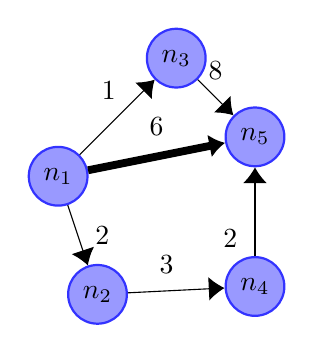
\begin{tikzpicture}
                \tikzset{Node/.style={circle, thick, draw=blue!80, fill=blue!40, minimum size=0.5cm}}
                \tikzset{OptimalPath/.style={circle, thick, draw=blue!80, fill=blue!40, minimum size=0.5cm}}
        
                \node[Node](N01) at (1.5,5) {$n_{1}$};
                \node[Node](N02) at (2,3.5) {$n_{2}$};
                \node[Node](N03) at (3,6.5) {$n_{3}$};
                \node[Node](N04) at (4,3.6) {$n_{4}$};
                \node[Node](N05) at (4,5.5) {$n_{5}$};
        
                \draw[-{Latex[length=2mm,width=3mm]}]
                    (N01) edge node[above=1mm,xshift=-3pt]{$1$} (N03) 
                    (N03) edge node[above=1mm]{$8$} (N05)
                    (N01) edge node[right=1mm]{$2$} (N02) 
                    (N04) edge node[pos=0.2,left=1mm]{$2$} (N05)
                    (N02) edge node[pos=0.4,above=1mm]{$3$} (N04)
                ;

                \draw[-{Latex[length=2mm,width=3mm]}, line width=1mm]
                    (N01) edge node[above=1mm]{$6$} (N05) 
                ;
            \end{tikzpicture}
            \caption{original graph}
            \label{fig:pathfinding:idea:single edgecostschanges:a}
        \end{subfigure}\quad%
        \begin{subfigure}{0.45\linewidth}
            \centering
            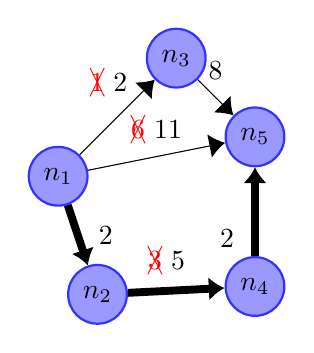
\begin{tikzpicture}
                \tikzset{Node/.style={circle, thick, draw=blue!80, fill=blue!40, minimum size=0.5cm}}
                \tikzset{OptimalPath/.style={circle, thick, draw=blue!80, fill=blue!40, minimum size=0.5cm}}
        
                \node[Node](N01) at (1.5,5) {$n_{1}$};
                \node[Node](N02) at (2,3.5) {$n_{2}$};
                \node[Node](N03) at (3,6.5) {$n_{3}$};
                \node[Node](N04) at (4,3.6) {$n_{4}$};
                \node[Node](N05) at (4,5.5) {$n_{5}$};
        
                \draw[-{Latex[length=2mm,width=3mm]}]
                    (N01) edge node[above=2mm,xshift=-3pt]{{\color{red} $\xcancel{1}$} $2$} (N03) 
                    (N03) edge node[above=1mm]{$8$} (N05)
                    (N01) edge node[above=1mm]{{\color{red} $\xcancel{6}$} $11$} (N05) 
                ;

                \draw[-{Latex[length=2mm,width=3mm]}, line width=1mm]
                    (N01) edge node[right=1mm]{$2$} (N02) 
                    (N02) edge node[pos=0.4,above=1mm]{{\color{red} $\xcancel{3}$} $5$} (N04)
                    (N04) edge node[pos=0.2,left=1mm]{$2$} (N05)
                ;
            \end{tikzpicture}
            \caption{Graph temporary altered}
            \label{fig:pathfinding:idea:single edgecostschanges:b}
        \end{subfigure}%
    \end{figure}
\end{frame}

\begin{frame}{A Motivating Example (2)}
    We can solve it:
    \begin{itemize}
        \item 4 Algorithms: Dijkstra, \code{ALT}, A* + Euclidean Distance, A* + CPD, \textbf{CPD search} (our technique!);
        \item On which map? hrt201, dustwallowkeys, mazes512-1-4, rooms16-003, ...;
        \item How to generate perturbations? \textbf{R}andomly? If so how many \textbf{E}dges should we affect? Or by affecting a specific \textbf{A}rea along the optimal path? If so, how \textbf{W}ide the area is? Where should we affect the \textbf{P}ath?
    \end{itemize}
\end{frame}

\begin{frame}{A Motivating Example (3)}
    \begin{figure}
        \centering
        \begin{subfigure}{0.49\textwidth}
            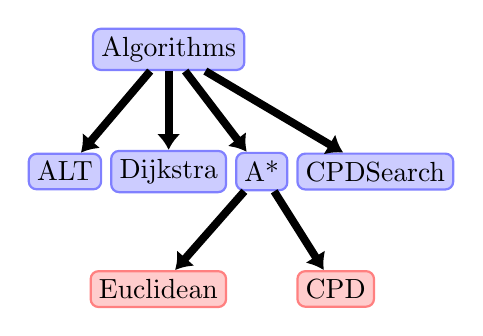
\begin{tikzpicture}
                \tikzstyle{vertex} = [shape=rectangle, rounded corners=1mm, draw=blue!50, fill=blue!20, thick, minimum size=3mm, inner sep=3pt, node distance=1.0cm and 0.1cm];
                \tikzstyle{vertex2} = [shape=rectangle, rounded corners=1mm, draw=red!50, fill=red!20, thick, minimum size=3mm, inner sep=3pt, node distance=1cm and 0.1cm];
    
                \node[vertex](Algorithms) at (0,0) {Algorithms};
                \node[vertex, below =of Algorithms](Dijkstra) {Dijkstra};
                \node[vertex, left =of Dijkstra](ALT) {ALT};
                \node[vertex, right =of Dijkstra](Astar) {A*};
                \node[vertex, right =of Astar](CPDSearch) {CPDSearch};
                \node[vertex2, below left =of Astar](Euclidean) {Euclidean};
                \node[vertex2, below right =of Astar](CPD) {CPD};
    
                \draw[-{Latex[length=2mm,width=3mm]}, line width=1mm]
                    (Algorithms) edge node[]{} (Dijkstra) 
                    (Algorithms) edge node[]{} (ALT) 
                    (Algorithms) edge node[]{} (Astar) 
                    (Algorithms) edge node[]{} (CPDSearch)
                    (Astar) edge node[]{} (Euclidean)  
                    (Astar) edge node[]{} (CPD) 
                ;
            \end{tikzpicture}
        \end{subfigure}\hfill%
        \begin{subfigure}{0.49\textwidth}
            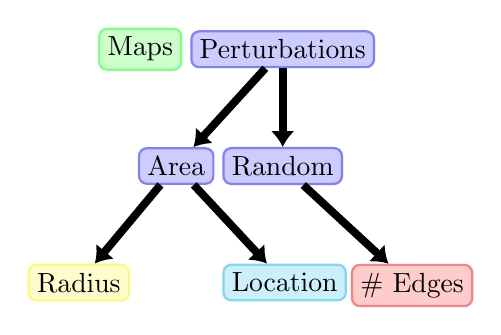
\begin{tikzpicture}
                \tikzstyle{vertex} = [shape=rectangle, rounded corners=1mm, draw=blue!50, fill=blue!20, thick, minimum size=3mm, inner sep=3pt, node distance=1.0cm and 0.1cm];
\tikzstyle{vertex2} = [shape=rectangle, rounded corners=1mm, draw=red!50, fill=red!20, thick, minimum size=3mm, inner sep=3pt, node distance=1cm and 0.1cm];
\tikzstyle{vertex3} = [shape=rectangle, rounded corners=1mm, draw=green!50, fill=green!20, thick, minimum size=3mm, inner sep=3pt, node distance=1cm and 0.1cm];
\tikzstyle{vertex4} = [shape=rectangle, rounded corners=1mm, draw=yellow!50, fill=yellow!20, thick, minimum size=3mm, inner sep=3pt, node distance=1cm and 0.1cm];
\tikzstyle{vertex5} = [shape=rectangle, rounded corners=1mm, draw=cyan!50, fill=cyan!20, thick, minimum size=3mm, inner sep=3pt, node distance=1cm and 0.1cm];

\node[vertex3](Maps) at (0,0) {Maps};
\node[vertex, right=of Maps](Perturbations) {Perturbations};
\node[vertex, below =of Perturbations](Random) {Random};
\node[vertex, left =of Random](Area) {Area};
\node[vertex2, below right =of Random](Edges) {\# Edges};
\node[vertex4, below left =of Area](Radius) {Radius};
\node[vertex5, below right=of Area](Location) {Location};

\draw[-{Latex[length=2mm,width=3mm]}, line width=1mm]
    (Perturbations) edge node[]{} (Random) 
    (Perturbations) edge node[]{} (Area) 
    (Random) edge node[]{} (Edges) 
    (Area) edge node[]{} (Radius)
    (Area) edge node[]{} (Location)  
;
            \end{tikzpicture}
        \end{subfigure}%
    \end{figure}
\end{frame}

\begin{frame}{A Motivating Example (4)}
    \begin{figure}
        \centering
        \begin{subfigure}{0.45\textwidth}
            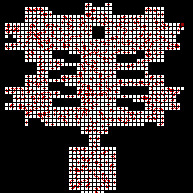
\includegraphics[width=1.0\textwidth]{{src/images/random}}
        \end{subfigure}\hfill%
        \begin{subfigure}{0.45\textwidth}
            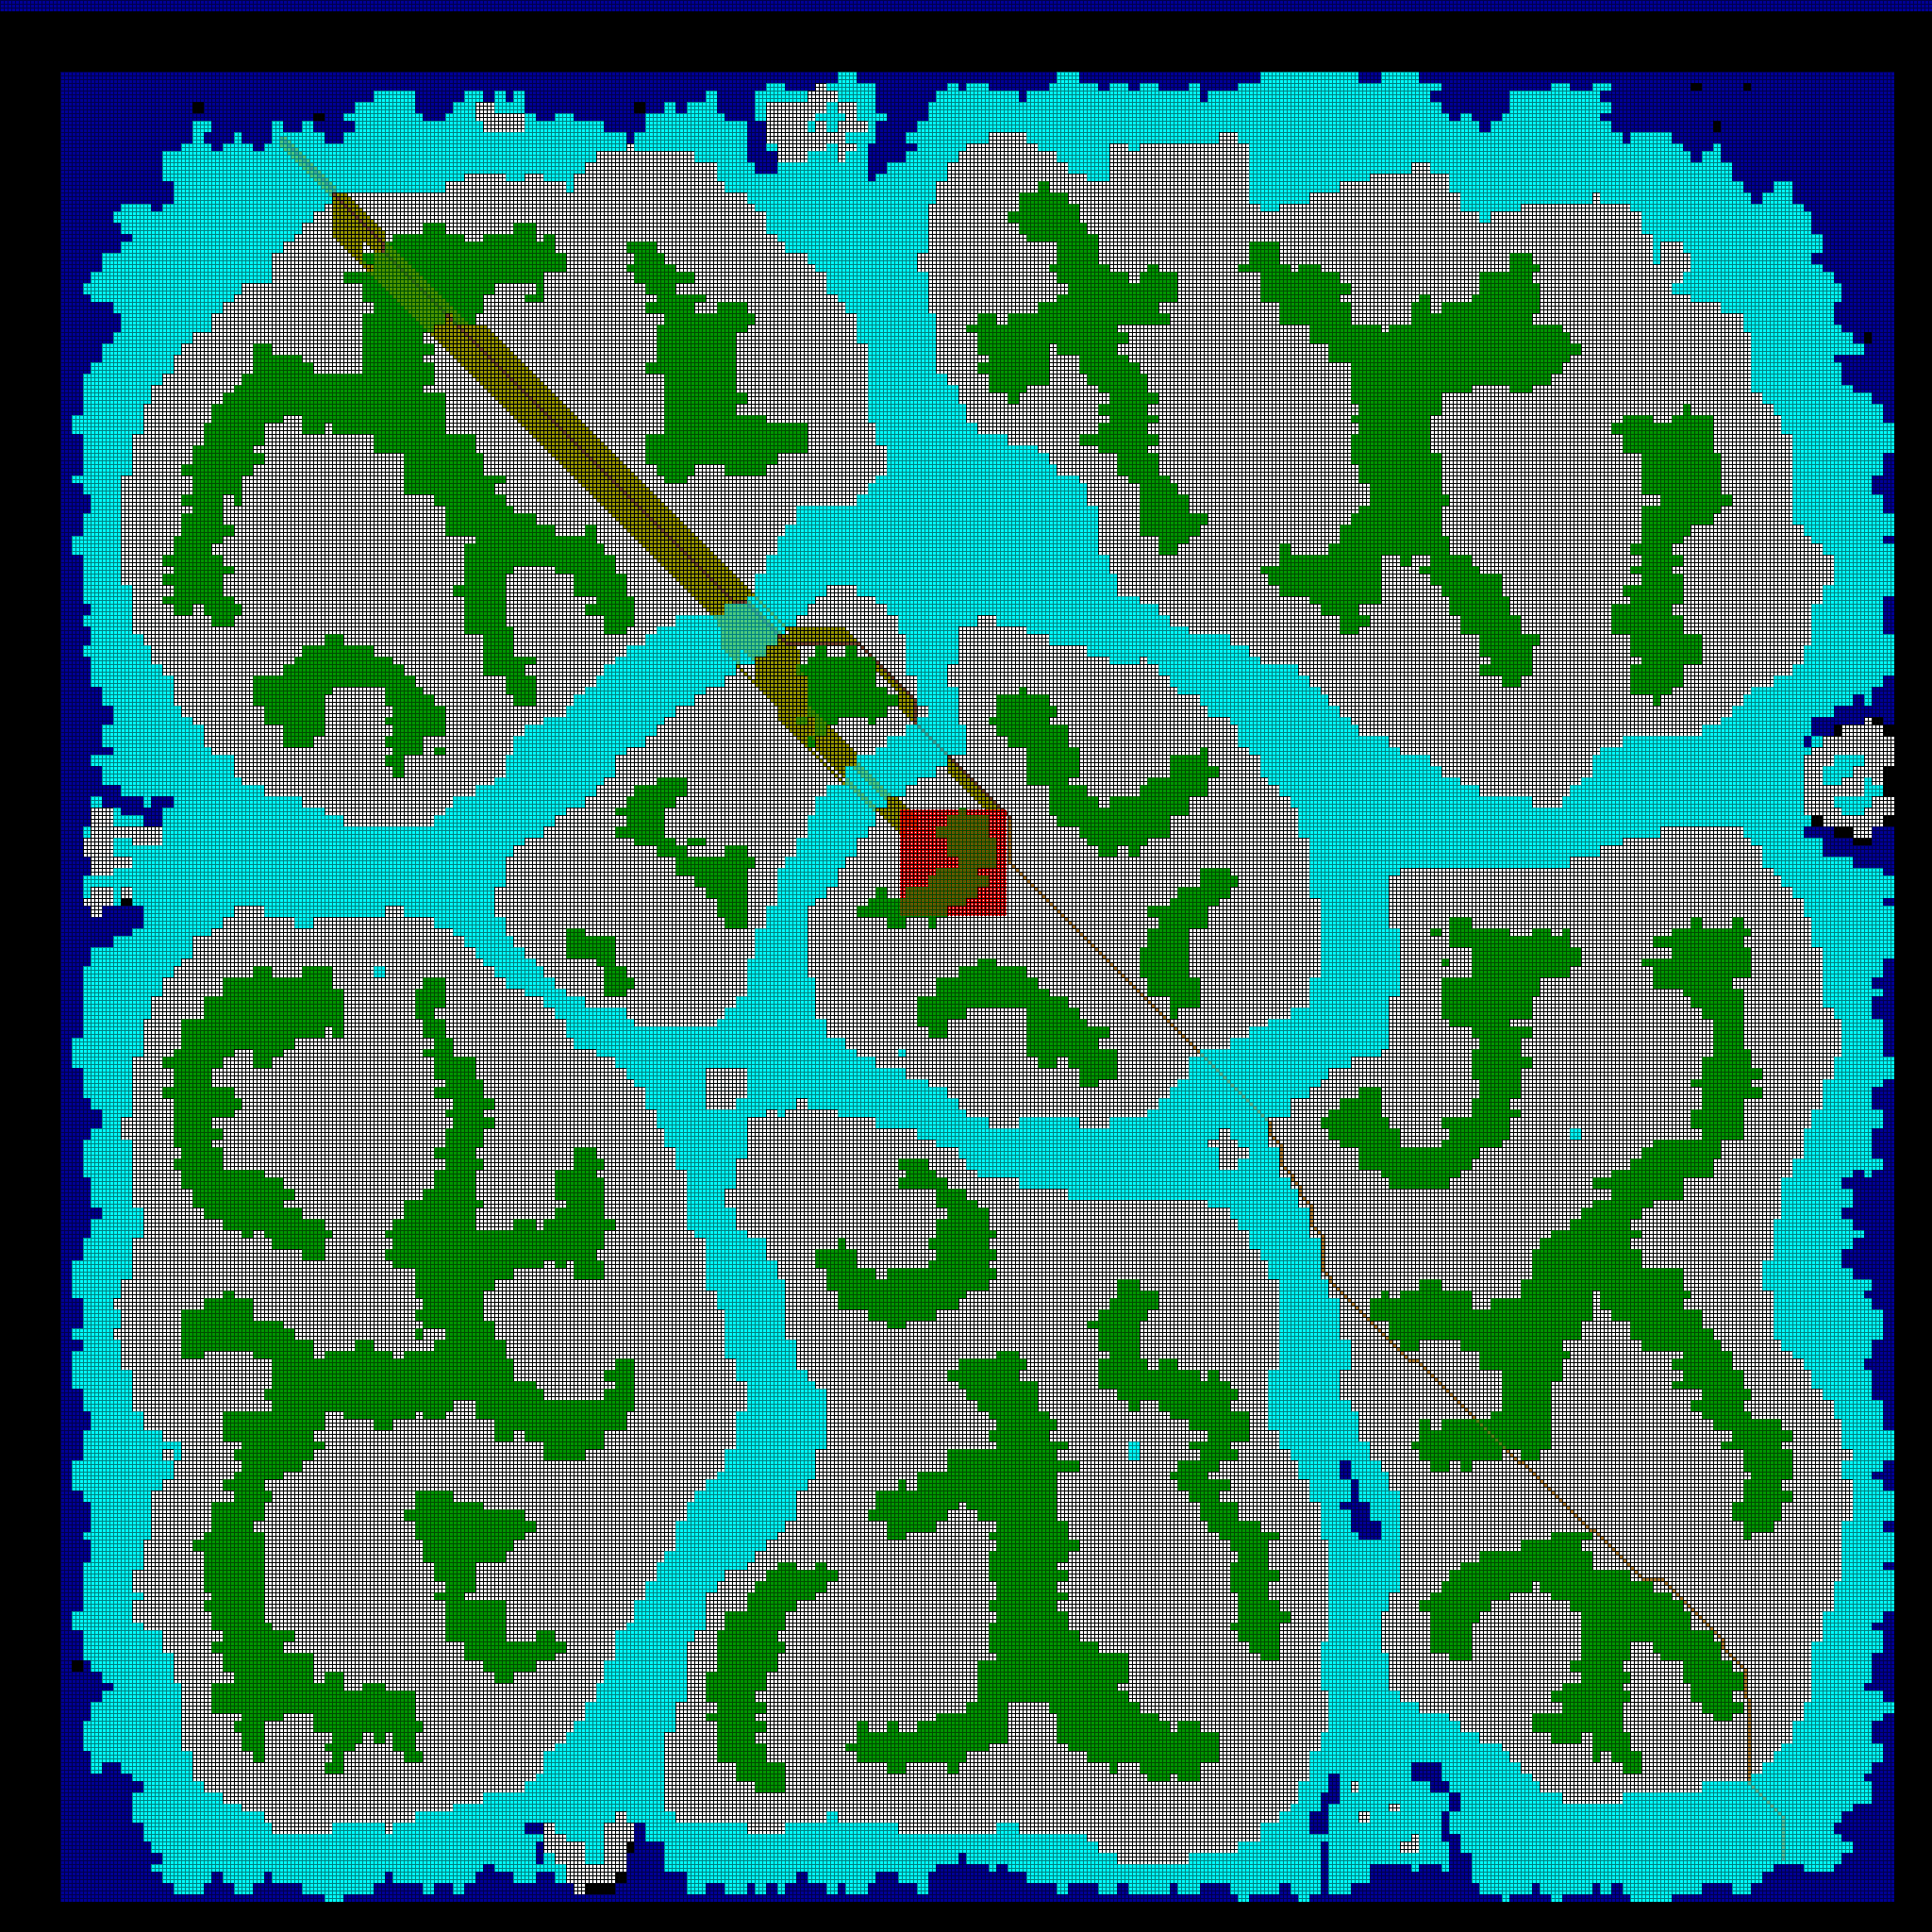
\includegraphics[width=1.0\textwidth]{{src/images/area}}
        \end{subfigure}%
        \caption{Example of perturbation policies. perturbations are shown in red. Left: random; Right: area}
    \end{figure}
\end{frame}

\begin{frame}{A Motivating Example (5)}
    $$|Algs| = 5, |Maps| = 4, |Perturbations| = 2$$ 
    $$\Downarrow$$
    $$Algs \times Maps \times Perturbations = 32$$

    But \textbf{R} depends on parameter \textbf{E} while \textbf{A} depends on \textbf{W} and \textbf{P} parameters!

    If we can choose the parameters:
    \begin{itemize}
        \item[-] $E \in \{1\%, 5\%, 10\% \}$;
        \item[-] $P \in \{20\%, 50\%, 100\% \}$;
        \item[-] $W \in \{5, 10, 15 \}$; 
    \end{itemize}
    
    Maximum combinations: $32 \cdot |E \times P \times W| = 864$!
    If we add new parameters (which, in research, it happens quite often) maximum combinations significantly increases!
\end{frame}

\begin{frame}{Talk Outline}
    The talk will be outlined as follows:
    \begin{itemize}
        \item Background: Software and design patterns used;
        \item Proposed Technique: \code{KS001}, \code{phd-tester} and the general framework flow;
        \item Conclusion and Future Works: integration with \code{CSPs} and generates automatic report pdf;
    \end{itemize}
\end{frame}
\section*{Background}

\begin{frame}{CSV file format}
    \begin{minipage}{0.40\textwidth}
        \begin{itemize}
            \item[-] Easy for storing data in \dquote{tabular} format;
            \item[-] Human readable;
            \item[-] can be read by tabular softwares (\ie{} Excel, LibreOffice Calc);  
        \end{itemize}
    \end{minipage}\hfill%
    \begin{minipage}{0.59\textwidth}
        \begin{figure}
            \centering
            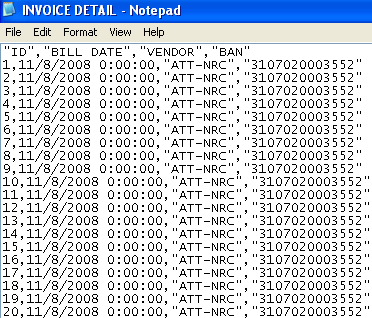
\includegraphics[width=1.0\textwidth]{{src/images/csv}}
        \end{figure}
    \end{minipage}%
\end{frame}

\begin{frame}{Background and technologies used}

    \begin{minipage}{0.48\textwidth}
        \begin{itemize}
            \item Language: Python 3[.6]: duck typing, scripting, \code{ABC} library, usually installed by default;
            \item ArangoDB: NoSQL graph-based database; basically we can store \code{JSON}; Compactly represent data;
            \item Pandas: allows operations on \dquote{dataframe} ($\approx$ CSV);
        \end{itemize}
    \end{minipage}\hfill%
    \begin{minipage}{0.48\textwidth}
        \begin{figure}
            \centering
            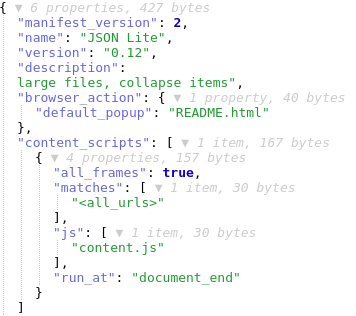
\includegraphics[width=1.0\textwidth]{{src/images/json}}
        \end{figure}
    \end{minipage}%

\end{frame}

\begin{frame}{Design Patterns}
    \begin{itemize}
        \item template: abstract class provides general behaviour with an concrete unmodifiable method $m$ whilst derived classes implements single tasks used in $m$ (\eg{} \code{java.awt.Component});
        \item Interface: allows usage of methods from a not-well specified object abstracting from its actual implementation;
        \item API: a method or a service a library or a third-party system provides to the developer in order to perform a task;
    \end{itemize}
\end{frame}
\section*{\code{phd-tester}}

\begin{frame}{Main Ideas}
    \begin{block}{\phantom{}}
    Each \textbf{test} $t \in \mathcal{T}$ involves a \textbf{stuff} $s \in \mathcal{S}$ to test (\eg{} algorithm) and an \textbf{environment} $e \in \mathcal{E}$ where the test occurs (\eg{} path finding map) Each \textbf{stuff}(\textbf{environment}) is a tuple of $n$($m$) values of parameters $p_i \in \mathcal{P}$ (\eg{} number of edge to perturbate, heuristic to use), where each parameter value $v_i$ has a specific domain $\mathcal{D}_{i} \cup \{nil \}$ (NIL). All Elements in $\mathcal{S}$($\mathcal{E}$) share the same tuple structure.
    \end{block}
    \vspace{-5pt}
    \begin{block}{\phantom{}}
        The final application is composed by 2 parts:
        \begin{enumerate}
            \item a \textbf{library} which the user call and provide a \textit{template design pattern} with easy APIs (provided by \code{phd-tester});
            \item a \textbf{user code} which implements the \textit{template design pattern}, providing mandatory information about the test as well as actually call the program to test (pro: test can be coded with any language!).
        \end{enumerate}
    \end{block}
    
\end{frame}

\begin{frame}{Template to follow}
    High-level steps in the \textit{template} provided by the framework:
    \begin{enumerate}
        \item the user specifies all the parameter values he wants (\eg{} perturbation generation policy $\in \{ \mbox{random}, \mbox{area} \}$);
        \item the application generates all the required tests $\mathcal{T}^{*} \subseteq \mathcal{T}$;
        \item the application executes all the tests $t \in \mathcal{T}^{*}$;
        \item the application produces generate $n$ CSVs representing test outcome (note $n \geq |\mathcal{T}^{*}|$);
    \end{enumerate}
\end{frame}

\begin{frame}{Option Graph}
    \begin{block}{\hphantom{}}
        The user specifies all the parameter values he wants (\eg{} perturbation generation policy $\in \{ \mbox{random}, \mbox{area} \}$);
    \end{block}

    \begin{minipage}{0.49\textwidth}
        By command line. In order to build the CLI interface, developer needs in \textit{user code} to declare the \textbf{option graph}: $\forall p_i \in \mathcal{P}$ say its domain $\mathcal{D}_i$, and what constraints it implies (\eg{} if parameter \code{perturbationPolicy} is set to \code{random}, then the CLI needs to specify parameter value \code{edge number}).
    \end{minipage}\hfill%
    \begin{minipage}{0.49\textwidth}
        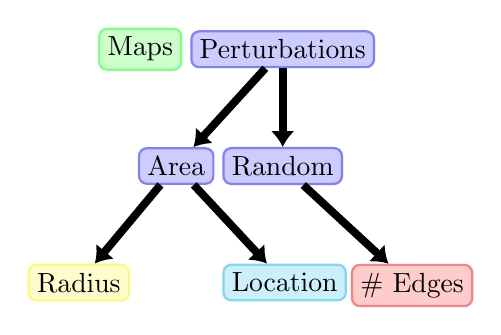
\begin{tikzpicture}
            \tikzstyle{vertex} = [shape=rectangle, rounded corners=1mm, draw=blue!50, fill=blue!20, thick, minimum size=3mm, inner sep=3pt, node distance=1.0cm and 0.1cm];
\tikzstyle{vertex2} = [shape=rectangle, rounded corners=1mm, draw=red!50, fill=red!20, thick, minimum size=3mm, inner sep=3pt, node distance=1cm and 0.1cm];
\tikzstyle{vertex3} = [shape=rectangle, rounded corners=1mm, draw=green!50, fill=green!20, thick, minimum size=3mm, inner sep=3pt, node distance=1cm and 0.1cm];
\tikzstyle{vertex4} = [shape=rectangle, rounded corners=1mm, draw=yellow!50, fill=yellow!20, thick, minimum size=3mm, inner sep=3pt, node distance=1cm and 0.1cm];
\tikzstyle{vertex5} = [shape=rectangle, rounded corners=1mm, draw=cyan!50, fill=cyan!20, thick, minimum size=3mm, inner sep=3pt, node distance=1cm and 0.1cm];

\node[vertex3](Maps) at (0,0) {Maps};
\node[vertex, right=of Maps](Perturbations) {Perturbations};
\node[vertex, below =of Perturbations](Random) {Random};
\node[vertex, left =of Random](Area) {Area};
\node[vertex2, below right =of Random](Edges) {\# Edges};
\node[vertex4, below left =of Area](Radius) {Radius};
\node[vertex5, below right=of Area](Location) {Location};

\draw[-{Latex[length=2mm,width=3mm]}, line width=1mm]
    (Perturbations) edge node[]{} (Random) 
    (Perturbations) edge node[]{} (Area) 
    (Random) edge node[]{} (Edges) 
    (Area) edge node[]{} (Radius)
    (Area) edge node[]{} (Location)  
;
        \end{tikzpicture}
    \end{minipage}
\end{frame}

\begin{frame}{Example of Option graph}
    \begin{figure}
        \begin{subfigure}{1.0\textwidth}
            \centering
            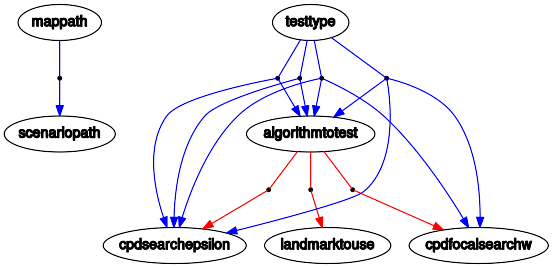
\includegraphics[width=0.9\textwidth]{src/images/optionGraph1.png}
        \end{subfigure}\\
        \begin{subfigure}{1.0\textwidth}
            \centering
            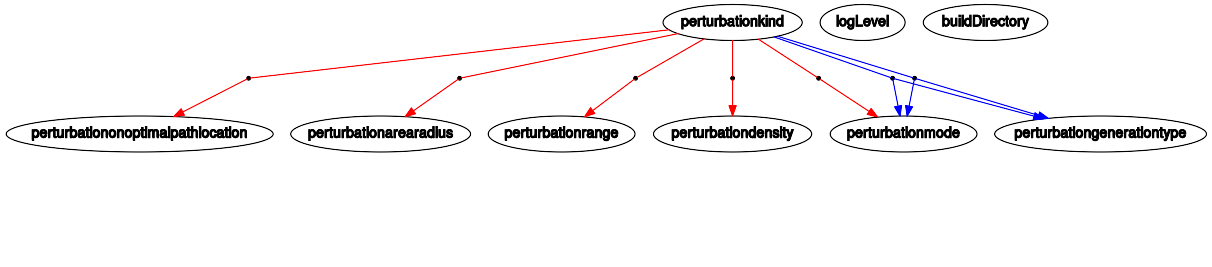
\includegraphics[width=1.09\textwidth]{src/images/optionGraph2.png}
        \end{subfigure}
    \end{figure}
\end{frame}

\begin{frame}{CLI generated}
    \begin{figure}
        \centering
        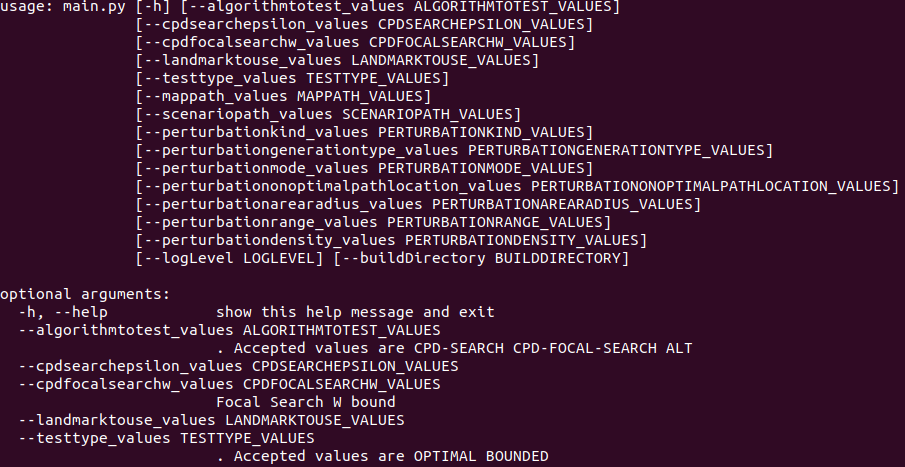
\includegraphics[width=1.0\textwidth]{src/images/help.png}
    \end{figure}
\end{frame}

\begin{frame}{Generation of $\mathcal{T}^{*}$}
    \begin{block}{\hphantom{}}
        the application generates all the required tests $\mathcal{T}^{*} \subseteq \mathcal{T}$.
    \end{block}

    $\mathcal{T}^{*}$ represents all the tests which we are required to execute. Some cartesian products in $\mathcal{S} \times \mathcal{E}$ are simply invalid (\eg{} \code{number of edges} to perturbate set to $\squote{nil}$ when the \code{perturbation policy} is $random$).

    \code{phd-tester} exploits the option graph not only to generate the CLI, but also to detect parameters dependencies.
    
    \textbf{Example:} Given a $t \in \mathcal{T}$ if \code{perturbation policy} is $random$, require that \code{number of edges}$\not = \squote{nil}$: if it is true, add $t$ in $\mathcal{T}^{*}$).
\end{frame}

\begin{frame}{Execute tests}

    \begin{block}{\hphantom{}}
        The application produces generate $n$ CSVs representing test outcome (note $n \geq |\mathcal{T}^{*}|$);
    \end{block}

    In this step the \textbf{user code} has all the freedom it desires. Usually the developer is expected to call an external program (\eg{} coded in \code{C} or in \code{C++}) that actually performs the test. As a side effect, one or more CSVs are expected to be produced somewhere (\ie{} file system, ArangoDB, mySQL $\Rightarrow$ \textbf{Data source}).

    \begin{itemize}
        \item \textbf{Problem:} how to identify which CSVs have been generated by which test $t \in \mathcal{T}^{*}$?
        \item \textbf{Solution:} by creating a new naming convention of file: \code{KS001};
    \end{itemize}
\end{frame}

\begin{frame}{\code{KS001} standard}
    \vspace{-9pt}
    \begin{block}{Idea}
        The filename is composed by \code{basename} and \code{extension}. \code{basename} is a \textbf{ordered} sequence of substring separated by \code{|}, and it is optionally prefixed by a \code{label}. Each substring is a unordered sequence of keyvalues string, separated by \code{\_}. Each keyvalue follows the pattern \code{key=value}.
    \end{block}
    \vspace{-3pt}
    \begin{figure}[h]
        \centering
        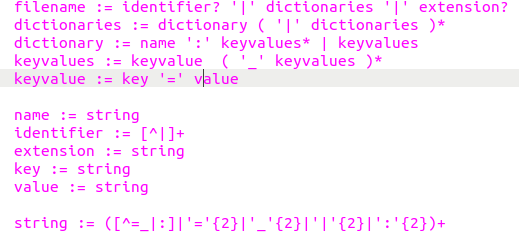
\includegraphics[width=1.0\textwidth]{src/images/ks001.png}
    \end{figure}
\end{frame}

\begin{frame}{Example of \code{KS001}}
    
    \begin{block}{\hphantom{}}
        \code{%
            |{\color{red}mp}=16room\_\_003.map\_pd=0.1\_pgt=PER-SCENARIO\_pk=RANDOM
            \_pm=MULTIPLY\_pr=[3,3]\_sp={\color{blue!50!green!50}16room\_\_003.map.scen}
            |{\color{blue}generated}:type=id-over-time|{\color{orange}.csv}
        }
    \end{block}

    \begin{itemize}
        \item doubling special characters if shown in key(value);
        \item aliasing of key(values) to avoid long names (you may reach path size limit);
        \item labelling of dictionary increase readability;
        \item \code{phd-tester} offers a set of function to query and manage \code{KS001} compliant strings;
    \end{itemize}
    
\end{frame}

\begin{frame}{Generation of interesting data (1)}
    \begin{block}{\hphantom{}}
        The application produces generate $n$ CSVs representing test outcome (note $n \geq |\mathcal{T}^{*}|$);
    \end{block}

    We use all the CSVs produced in the previous phase and stored in a \textbf{data source} to generate \textit{new} CSVs representing the benchmarks (and optionally, the related graphs as well).

    \begin{figure}
        \centering
        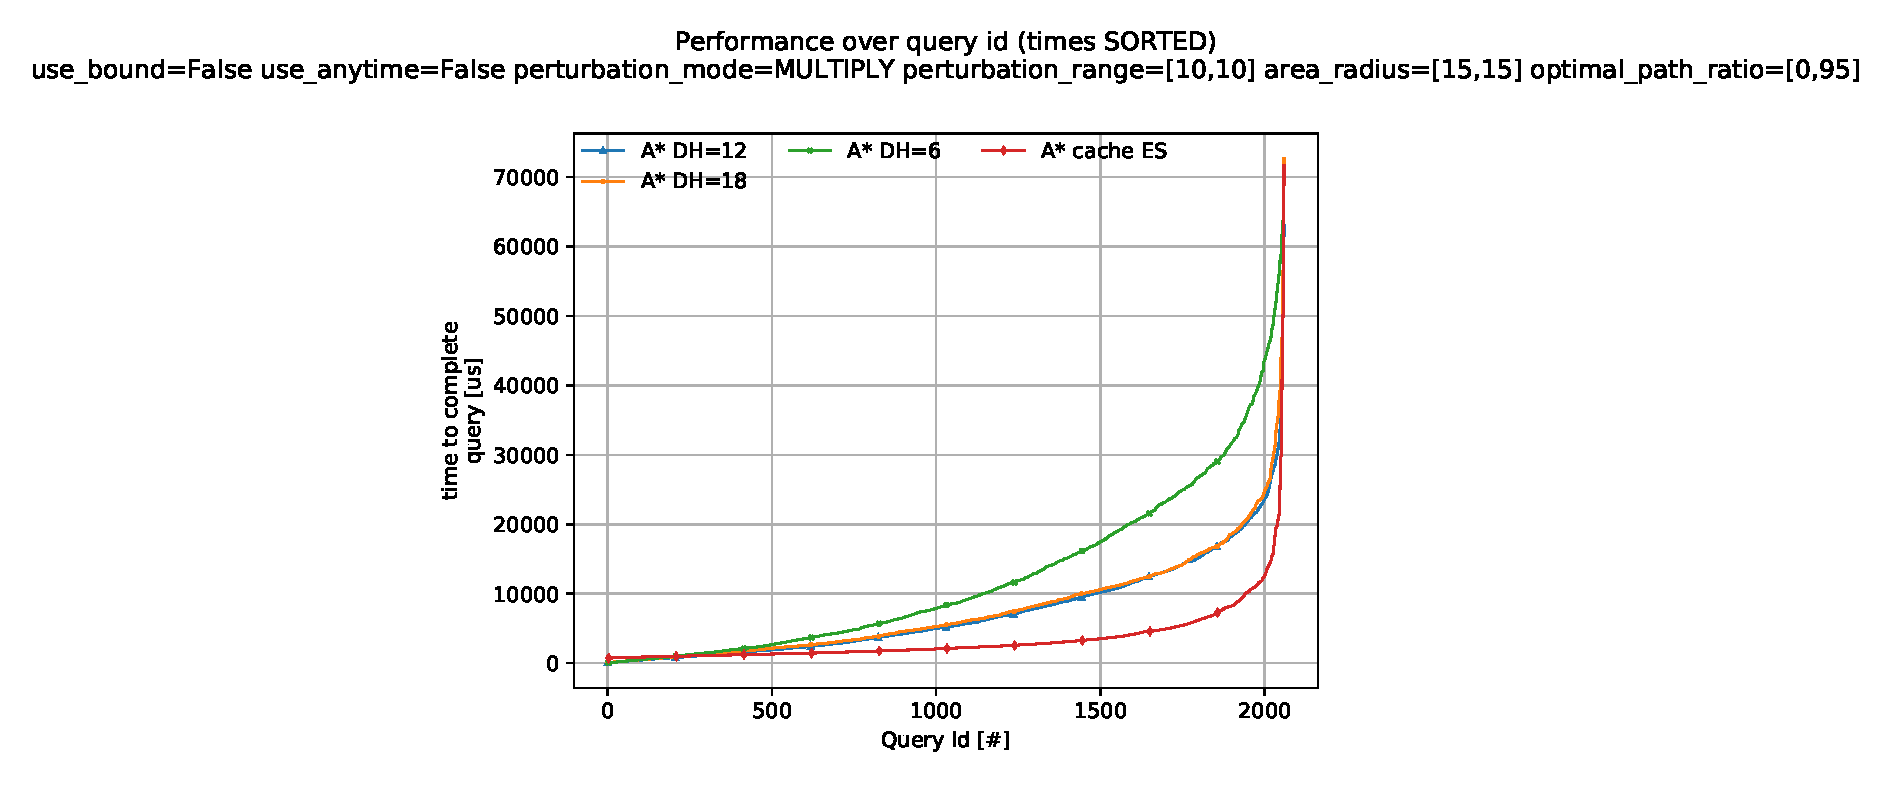
\includegraphics[width=1.0\textwidth]{src/images/example.eps}
    \end{figure}
\end{frame}

\begin{frame}{Generation of interesting data (2)}
    \code{phd-tester} dynamically generate these csv(image).

    \begin{itemize}
        \item each csv(image) is often produced by analyzing one or more outputs of tests in $\mathcal{T}^{*}$;
        \item \code{phd-tester} provides \textbf{masks}, which acts as filter allowing the software to fetch a subset of $\mathcal{T}^{*}$ to consider to produce a new csv(image) (\eg{} produce time used by all algorithm depending on the number of edge perturbated in the map);
        \item The number of CSVs to analyze may be huge (maybe over 30000, each with 100 an more rows!). \code{phd-tester} used \code{pandas} along with \code{dask} to concurrently computes the operations $\Rightarrow$ fast;
        \item \code{CurveChanger}: allows to further alters the functions generated by adding/removing/sorting values;
    \end{itemize}
\end{frame}



\section*{Conclusions}

\begin{frame}{Conclusions and Future Works}
    In conclusion:
    \begin{itemize}
        \item We have developed \code{phd-tester}, an extensible framework to combinatorially testing algorithms, parametrized both in regard of what we're testing and of the environment of the test;
        \item proposed a naming convention of files which is both human readable and software parsable (\code{KS001});
        \item developed a mechanism to concurrently computed generated data and plot it;
        \item \textbf{Future works:} integrate MySQL as data source; generate automatic pdf reports of the tests done; Use a CSP to build the option graph. See \code{https://github.com/Koldar/phdTester/issues} for further works to be done.
    \end{itemize}
\end{frame}

\end{document}
